\documentclass[conference]{IEEEtran}
\IEEEoverridecommandlockouts
\usepackage{cite}
\usepackage{amsmath,amssymb,amsfonts}
\usepackage{graphicx}
\usepackage{textcomp}
\usepackage{xcolor}
\usepackage{booktabs}
\usepackage{array}
\usepackage{enumitem}
\usepackage{tikz}
\usetikzlibrary{arrows.meta,positioning}

\newcommand{\sat}{\operatorname{sat}}
\newcommand{\sign}{\operatorname{sign}}
\newcommand{\diag}{\operatorname{diag}}

\begin{document}

\title{Quanser Aero~2 Twin-Rotor System:\\ Hardware Physics, Identification, Modelling, and the Complete Controller Suite\\
{\footnotesize Mathematical foundations for offline simulation, digital-twin, and hardware execution}}

\author{\IEEEauthorblockN{Gandhi Contreras}
\IEEEauthorblockA{\textit{Electrical and Computer Engineering}, New Mexico State University, Las Cruces, NM, USA \\ gandhico@nmsu.edu}}

\maketitle

\begin{abstract}
This paper consolidates the complete mathematics of the Quanser Aero~2 two-degree-of-freedom twin-rotor platform, from the wall supply to the closed control loop. The hardware physics are developed explicitly: the PWM amplifier, the two DC motor--propeller assemblies with their aerodynamic thrust and reaction-torque maps, the pitch/yaw encoders, the MEMS inertial unit with measured bias and noise statistics, and the sampled USB loop whose \emph{measured} period --- not its commanded one --- must drive every discrete update. The implemented nonlinear model (drift plus state-dependent input matrix with a yaw-authority cosine bound), its linearization, and the collective/differential input decomposition are derived and tied to physical parameters. The identification chapter formulates the excitation design, ARX/DARX least squares, and the validated result that the identified models are strong one-step predictors and weak free-run simulators --- a distinction preserved rather than averaged away. The controller suite is then developed with the exact implemented parameterizations: PD with second-order filtered derivatives, LQR with least-squares feedforward, LQG, unconstrained finite-horizon linear MPC, backstepping and sliding-mode control through least-squares inverse dynamics, and a real-time nonlinear MPC. Hardware-validated benchmark conclusions and the safety envelope complete the treatment.
\end{abstract}

\begin{IEEEkeywords}
Quanser Aero 2, twin rotor, hardware physics, ARX identification, PD, LQR, LQG, MPC, backstepping, sliding-mode control, NMPC, digital twin.
\end{IEEEkeywords}

%====================================================================
\section{Introduction}
The Aero~2 is a table-top twin-rotor aircraft: two propeller assemblies at the ends of a beam that pitches ($\theta$) about a horizontal axis and yaws ($\psi$) about the vertical. Both axes are excited by both rotors, making it a genuinely coupled two-input two-output plant with trim sensitivity, yaw stiction, actuator saturation, and real-time timing effects. The state, input, and output conventions used by all of our implementations are
\begin{equation}
x = [\theta,\ \dot\theta,\ \psi,\ \dot\psi]^{\!\top},\quad
u = [u_p,\ u_y]^{\!\top},\quad
y = [\theta,\ \psi]^{\!\top},
\end{equation}
where $(u_p,u_y)$ are virtual pitch/yaw voltage commands mapped to the physical motor voltages $(v_0, v_1)$ by the mixer of Section~\ref{sec:mixer}. This paper presents the mathematics only --- hardware physics, identification, modelling, and control --- exactly as implemented and validated in our hardware campaigns; code, digital-twin software, and neuromorphic augmentation are treated elsewhere.

%====================================================================
\section{Hardware Physics: Energy Source to Aerodynamic Torque}\label{sec:hw}

\begin{figure*}[!t]
\centering
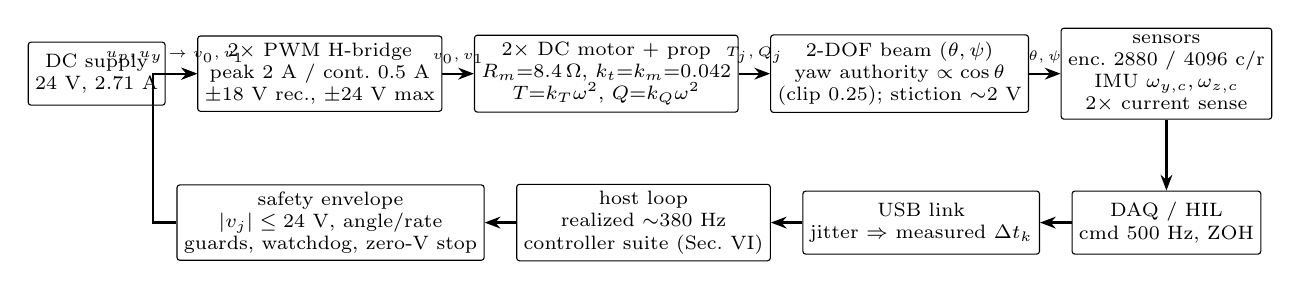
\begin{tikzpicture}[
  node distance=3mm and 4mm,
  blk/.style={draw, rounded corners=1pt, align=center, font=\scriptsize, inner sep=2.5pt, minimum height=8mm},
  lbl/.style={font=\tiny, align=center},
  arr/.style={-{Stealth[length=2mm]}, thick}
]

\node[blk] (sup) {DC supply\\ $24$ V, $2.71$ A};
\node[blk, right=of sup] (amp) {$2\times$ PWM H-bridge\\ peak 2 A / cont.\ 0.5 A\\ $\pm18$ V rec., $\pm24$ V max};
\node[blk, right=of amp] (mot) {$2\times$ DC motor + prop\\ $R_m{=}8.4\,\Omega$, $k_t{=}k_m{=}0.042$\\ $T{=}k_T\omega^2$, $Q{=}k_Q\omega^2$};
\node[blk, right=of mot] (mech) {2-DOF beam $(\theta,\psi)$\\ yaw authority $\propto\cos\theta$\\ (clip $0.25$); stiction $\sim$2 V};
\node[blk, right=of mech] (enc) {sensors\\ enc.\ 2880 / 4096 c/r\\ IMU $\omega_{y,c},\omega_{z,c}$\\ $2\times$ current sense};
\node[blk, below=9mm of enc] (daq) {DAQ / HIL\\ cmd 500 Hz, ZOH};
\node[blk, left=of daq] (usb) {USB link\\ jitter $\Rightarrow$ measured $\Delta t_k$};
\node[blk, left=of usb] (host) {host loop\\ realized $\sim$380 Hz\\ controller suite (Sec.~VI)};
\node[blk, left=of host] (safe) {safety envelope\\ $|v_j|\le24$ V, angle/rate\\ guards, watchdog, zero-V stop};
\draw[arr] (sup) -- (amp);
\draw[arr] (amp) -- node[lbl, above] {$v_0,v_1$} (mot);
\draw[arr] (mot) -- node[lbl, above] {$T_j,Q_j$} (mech);
\draw[arr] (mech) -- node[lbl, above] {$\theta,\psi$} (enc);
\draw[arr] (enc) -- (daq);
\draw[arr] (daq) -- (usb);
\draw[arr] (usb) -- (host);
\draw[arr] (host) -- (safe);
\draw[arr] (safe.west) -- ++(-3mm,0) |- node[lbl, pos=0.75, above] {$u_p,u_y \to v_0,v_1$} (amp.west);
\end{tikzpicture}
\caption{Aero~2 signal chain (amplifier/motor values verified against the user manual). The $\pm24$~V software clip is the amplifier's absolute output bound; every discrete update advances on the measured $\Delta t_k$.}
\label{fig:chain}
\end{figure*}

\subsection{Power path and amplifier}
A regulated external DC supply (24.0~V, up to 2.71~A per the user manual) powers the two motor drives; the USB link carries data. Each motor is driven by an H-bridge PWM stage; averaging over the switching period gives the terminal voltage $v_j = D_j V_s$, $D_j\in[-1,1]$. The manual-verified amplifier ratings are peak current 2~A, continuous current 0.5~A, recommended output $\pm18$~V, and \emph{maximum} output $\pm24$~V --- the physical origin of the software saturation $|v_j|\le V_{\max} = 24$~V used by every controller in this paper. Amplifier thermal behavior and supply droop under simultaneous high thrust on both rotors motivate the command-magnitude discipline of the safety envelope (Section~\ref{sec:safety}).

\subsection{Motor--propeller electromechanics and aerodynamics}
Each assembly is a DC motor spinning a fixed-pitch propeller. The armature satisfies $L_a\dot i + R_m i + k_m\omega = v$ with electromagnetic torque $k_t i$; manual-verified motor constants: $R_m = 8.4\,\Omega$, $k_t = 0.042$~N\,m/A, $k_m = 0.042$~V\,s/rad, $L_a = 1.16$~mH (so $\tau_e = L_a/R_m \approx 0.14$~ms, quasi-static at the loop rate), rotor inertia $4.0\times10^{-6}$~kg\,m$^2$, nominal 18~V / 0.54~A / 3050~RPM. The rotor speed obeys
\begin{equation}
J_\omega\dot\omega = k_t i - Q_a(\omega) - b_\omega\omega,
\label{eq:rotor}
\end{equation}
where the aerodynamic load is the propeller torque. Momentum theory for a propeller of radius $R$ in air of density $\rho$ gives the quasi-static maps
\begin{equation}
T_a = k_T\,\omega^2,\qquad Q_a = k_Q\,\omega^2,
\qquad k_T \!\propto\! \rho R^4,\; k_Q \!\propto\! \rho R^5,
\label{eq:aero}
\end{equation}
thrust normal to the rotor disc and reaction torque about its axis. The motor electrical pole and the rotor-speed lag \eqref{eq:rotor} are fast relative to the rigid-body dynamics (motor-speed step responses on this hardware settle an order of magnitude faster than the pitch response), so for control-oriented modelling the chain voltage$\,\to\,$speed$\,\to\,$thrust is absorbed into locally linear \emph{effectiveness constants} about the operating point:
\begin{equation}
\Delta T_j \approx c_{T}\,\Delta v_j,\qquad \Delta Q_j \approx c_{Q}\,\Delta v_j,
\label{eq:effectiveness}
\end{equation}
which is precisely what the identified constants $K_{PP},K_{PY},K_{YP},K_{YY}$ of Section~\ref{sec:model} are: voltage-to-angular-acceleration effectiveness including \eqref{eq:aero}, the moment arms, and the drive electronics. This absorption is the reason the plant must be \emph{identified about a trim point} (Section~\ref{sec:id}) rather than assembled purely from datasheet aerodynamics.

\subsection{Mechanism and torque generation}\label{sec:mixer}
The beam carries the two rotors at moment arm $d_t$ from the pitch axis. Physically: the \emph{sum} of thrusts pitches the beam; the \emph{difference} of thrusts (and the difference of reaction torques) yaws it, with the yaw component of thrust scaled by the beam attitude. This motivates the collective/differential decomposition of the physical voltages,
\begin{equation}
u_c = \tfrac12\,(v_0 + v_1),\qquad
u_d = \tfrac12\,(v_0 - v_1),
\label{eq:coll_diff}
\end{equation}
with $u_c$ primarily exciting pitch and $u_d$ primarily exciting yaw. The virtual commands map as $(u_p,u_y)\!\to\!(v_0,v_1)$ either directly (one motor per virtual channel, the mapping used in our final hardware benchmarks) or in mixed form $v_{0,1} = u_p \mp u_y$; both are linear maps whose composition with \eqref{eq:effectiveness} is absorbed by identification. Yaw exhibits \emph{breakaway stiction}: small $|u_d|$ produces no yaw motion at rest (first clear motion on our rig required $|u_d|\approx2$~V), a Coulomb-type friction fact that shaped the excitation design of Section~\ref{sec:id}.

\subsection{Sensors}
\subsubsection{Incremental encoders} pitch and yaw angles are measured by quadrature encoders,
\begin{equation}
\theta = \frac{2\pi\,n_\theta}{2880},\qquad
\psi = \frac{2\pi\,n_\psi}{4096},
\end{equation}
with quantization steps $2.18$ and $1.53$~mrad respectively; both are relative (zeroed at initialization).
\subsubsection{MEMS inertial unit} a three-axis gyroscope and accelerometer. The gyroscope measurement model is
\begin{equation}
\omega_{\mathrm{meas}} = \omega_{\mathrm{true}} + b_\omega + \eta_\omega,
\end{equation}
with the stationary calibration \emph{measured on this unit} (1414 samples, 100 Hz):
\begin{align}
b_\omega &= [\,+0.00985550,\ -0.01797350,\ -0.00718040\,]\ \mathrm{rad/s},\nonumber\\
\sigma_\omega &= [\,0.00143607,\ 0.00156495,\ 0.00168013\,]\ \mathrm{rad/s},
\label{eq:imu}
\end{align}
and accelerometer mean $[-0.585,\ -0.206,\ +9.830]\,$m/s$^2$ consistent with gravity plus mounting offsets. The bias-corrected body rates
\begin{equation}
\dot\theta \approx \omega_y - b_y,\qquad \dot\psi \approx \omega_z - b_z
\end{equation}
are the rate feedback signals: on this hardware the corrected gyro pitch rate is $\sim$59$\times$ smoother (RMS of successive differences) than the quantized encoder finite difference at 200 Hz, which is why gyro rates are preferred for derivative feedback while encoders provide the angles.
\subsubsection{Current sensors} per-motor current monitors expose the armature currents of \eqref{eq:rotor} for stall/health monitoring.

\subsection{Sampling, USB loop, and the measured-$\Delta t$ rule}
The interface samples at a commanded rate (500~Hz in our controller runs) with zero-order hold on the outputs, $v(t) = v_d(k)$, $t\in[kT_s,(k{+}1)T_s)$. The host loop is soft real time: our hardware logs show \emph{realized} mean rates near $380$~Hz for the full controller suite (and $\sim$303~Hz for real-time NMPC). The headline implementation rule of this platform, established empirically, is that every derivative filter and discrete integration must advance with the measured period $\Delta t_k$; using the nominal $T_s$ corrupts the derivative action enough to change controller rankings. All controllers below take $\Delta t_k$ as an input.

\subsection{Safety envelope}\label{sec:safety}
(i) $|v_j|\le24$~V hard clip; (ii) attitude guards $|\theta|\le\theta_{\mathrm{safe}}$, $|\psi|\le\psi_{\mathrm{safe}}$ with commanded zero on violation; (iii) rate guards on the corrected gyro signals; (iv) watchdog on stale samples; (v) zero-voltage shutdown and amplifier disable on any stop; (vi) trim discipline --- excitation records discard the first 3~s (spin-up transient) before use.

%====================================================================
\section{Nonlinear and Linear Modelling}\label{sec:model}

\subsection{Implemented nonlinear model}
The plant is modelled as two coupled rotational axes with drift and a state-dependent input matrix:
\begin{equation}
\begin{bmatrix}\ddot\theta\\ \ddot\psi\end{bmatrix}
= b(\theta,\dot\theta,\dot\psi) + M(\theta)\,u,
\qquad u = [u_p,\ u_y]^{\!\top},
\label{eq:aero_nl}
\end{equation}
\begin{equation}
b = \begin{bmatrix}
\bigl(-K_{SP}\sin\theta - D_P\,\dot\theta\bigr)/J_P\\[2pt]
\bigl(-D_Y\,\dot\psi\bigr)/J_Y
\end{bmatrix},
\end{equation}
\begin{equation}
M(\theta) = \begin{bmatrix}
d_t K_{PP}/J_P & d_t K_{PY}/J_P\\[2pt]
c_\theta K_{YP}/J_Y & c_\theta K_{YY}/J_Y
\end{bmatrix},
\quad c_\theta = \cos\theta,
\label{eq:Mtheta}
\end{equation}
with the implementation-critical bound $|c_\theta| \ge 0.25$ (clipped): the yaw control authority scales with the cosine of pitch --- the physical projection of differential thrust onto the yaw axis --- and the clip bounds the model's authority loss at large pitch. Parameters (identified/implemented values):
$d_t = 0.16743$~m, $K_{SP}=0.00744$, $D_P=0.00199$, $K_{PP}=0.00321$, $K_{PY}=0.00137$, $D_Y=0.00192$, $K_{YY}=0.00610$, $K_{YP}=-0.00319$ (note the negative cross sign),
$J_P = 0.02318850$, $J_Y = 0.02381042\ \mathrm{kg\,m^2}$.
These identified values are \emph{independently confirmed by the manufacturer}: the user manual lists pitch inertia $2.32\times10^{-2}$, yaw inertia $2.38\times10^{-2}$~kg\,m$^2$, and thrust displacement $0.168$~m, agreeing with the identified $J_P$, $J_Y$, and $d_t = 0.16743$~m to three significant figures --- the model is grounded in both data and datasheet. The gravitational restoring term $K_{SP}\sin\theta$ is weak, so pitch behaves \emph{near-integrating} about trim --- the single most consequential structural fact for identification (Section~\ref{sec:id}) and for why free-run simulation is hard.

\subsection{Inverse dynamics}
Nonlinear controllers require the input achieving a desired acceleration $a_d$. Because $M(\theta)$ can be poorly conditioned at large pitch, the implemented inversion is least squares with saturation, never a symbolic inverse:
\begin{equation}
u = \sat_{V_{\max}}\Bigl(\arg\min_{u}\ \bigl\|M(\theta)\,u - (a_d - b)\bigr\|_2\Bigr).
\label{eq:invdyn}
\end{equation}

\subsection{Linearization}
About $\theta=0$ ($c_\theta = 1$), $\dot x = Ax + Bu$, $y = Cx$ with
\begin{equation}
A = \begin{bmatrix}
0&1&0&0\\
-\frac{K_{SP}}{J_P}&-\frac{D_P}{J_P}&0&0\\
0&0&0&1\\
0&0&0&-\frac{D_Y}{J_Y}
\end{bmatrix},\;
B = \begin{bmatrix}
0&0\\
\frac{d_tK_{PP}}{J_P}&\frac{d_tK_{PY}}{J_P}\\
0&0\\
\frac{K_{YP}}{J_Y}&\frac{K_{YY}}{J_Y}
\end{bmatrix},
\label{eq:aeroAB}
\end{equation}
$C = [\,e_1\ e_3\,]^{\!\top}$. This pair is the backbone of the LQR/LQG/MPC designs; the yaw row of $B$ drops the cosine factor (its linearization at $\theta=0$), while the nonlinear controllers keep \eqref{eq:Mtheta}.

%====================================================================
\section{Identification}\label{sec:id}

\begin{figure}[!t]
\centering
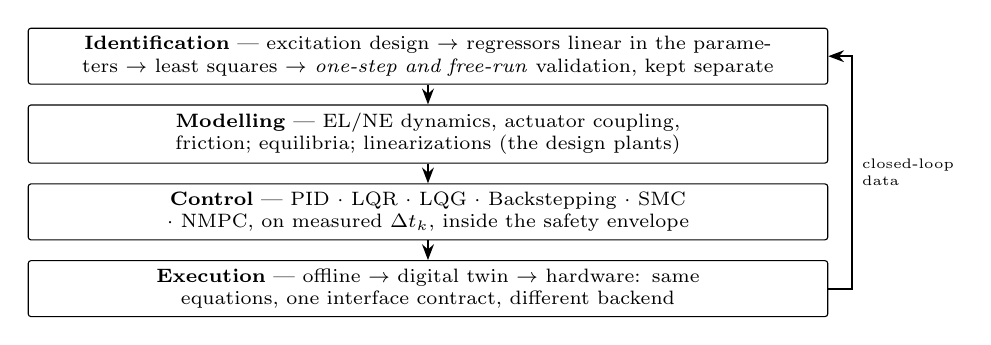
\begin{tikzpicture}[
  node distance=2.5mm,
  blk/.style={draw, rounded corners=1pt, align=center, font=\scriptsize, inner sep=3pt, text width=0.82\columnwidth},
  arr/.style={-{Stealth[length=2mm]}, thick}
]
\node[blk] (id) {\textbf{Identification} --- excitation design $\to$ regressors linear in the parameters $\to$ least squares $\to$ \emph{one-step and free-run} validation, kept separate};
\node[blk, below=of id] (mod) {\textbf{Modelling} --- EL/NE dynamics, actuator coupling, friction; equilibria; linearizations (the design plants)};
\node[blk, below=of mod] (ctl) {\textbf{Control} --- PID $\cdot$ LQR $\cdot$ LQG $\cdot$ Backstepping $\cdot$ SMC $\cdot$ NMPC, on measured $\Delta t_k$, inside the safety envelope};
\node[blk, below=of ctl] (exe) {\textbf{Execution} --- offline $\to$ digital twin $\to$ hardware: same equations, one interface contract, different backend};
\draw[arr] (id) -- (mod);
\draw[arr] (mod) -- (ctl);
\draw[arr] (ctl) -- (exe);
\draw[arr] (exe.east) -- ++(3mm,0) |- node[font=\tiny, pos=0.25, right, align=left] {closed-loop\\ data} (id.east);
\end{tikzpicture}
\caption{The workflow every platform in this series follows: identification feeds modelling, modelling feeds the controller suite, and all stages run unchanged across the three execution targets; closed-loop records return to identification.}
\label{fig:workflow}
\end{figure}

\subsection{Excitation design (dictated by the physics)}
\begin{enumerate}[label=E\arabic*)]
\item \emph{Trim search}: equal-voltage sweep of $u_c$; the practical operating point on our rig is $U_0 \approx 1.4$~V (pitch approximately neutral over short windows).
\item \emph{Pitch}: doublets and PRBS in common mode about trim, $v_0 = v_1 = U_0 + v_p$ with $|v_p|\approx0.075$~V --- small because pitch is near-integrating.
\item \emph{Yaw}: \emph{pure differential} drive $v_0 = -v_\psi$, $v_1 = +v_\psi$ with chirp amplitudes up to 6~V ($|v_0-v_1|\le12$~V): small differential inputs do not overcome breakaway, so yaw must be excited with authority. The informative yaw output is the bias-corrected gyro rate $\omega_{z,c}$, not the encoder angle (quantization-limited at small motion).
\item \emph{Coupled}: simultaneous collective + differential PRBS for the MIMO models. All records: discard $t<3$~s, remove means.
\end{enumerate}

\subsection{ARX/DARX least squares}
With regressor rows
$\varphi(k) = [\,1,\ y_{k-1},\dots,y_{k-n_a},\ u_{k-n_k},\dots,u_{k-n_k-n_b+1}\,]$
(per input channel in the MIMO case), the estimate is $\hat\beta = \arg\min\|\Phi\beta - Y\|_2$, and the discrete transfer form is $A(z^{-1})y_k = B(z^{-1})u_k + c$ with $A = 1 - a_1z^{-1} - \cdots$. The validated nominal models on this hardware are:
\begin{table}[h]
\caption{Identified DARX models (validation one-step fits)}
\centering
\begin{tabular}{lcccc}
\toprule
Case & Output & $T_s$ [s] & Order & Fit [\%]\\
\midrule
Pitch SISO & $\theta$ & 0.005571 & $n_a{=}1,n_b{=}3$ & 98.23\\
Yaw-rate SISO & $\omega_{z,c}$ & 0.005581 & $n_a{=}2,n_b{=}2,n_k{=}2$ & 91.43\\
Coupled pitch & $\theta$ & 0.011272 & $n_a{=}1,n_b{=}1$ & 99.26\\
Coupled yaw-rate & $\omega_{z,c}$ & 0.005610 & $n_a{=}3,n_b{=}4,n_k{=}2$ & 87.89\\
\bottomrule
\end{tabular}
\end{table}

\subsection{One-step versus free-run: the central result}
Validation on independent records distinguishes prediction from simulation. One-step fits are uniformly strong (pitch 97--99\%, yaw 87--91\%), while \emph{free-run} simulation is weak to very poor (yaw SISO 16.9\%; pitch and coupled cases diverge). The physics explains it: the near-integrating pitch channel accumulates small one-step errors without a restoring force. The identified models are therefore \emph{local predictive models} --- ideal for predictor-based control and validation --- and not long-horizon open-loop simulators; both figures are always reported, never averaged.

\subsection{Uncertainty for robust design}
Comparing identified and measured frequency responses yields the multiplicative uncertainty and fitted weight
\begin{equation}
\Delta_m(j\omega) = \frac{G_{\mathrm{meas}} - G_{\mathrm{nom}}}{G_{\mathrm{nom}}},\qquad
W_m(s) = k\,\frac{1 + s/\omega_z}{1 + s/\omega_p},
\end{equation}
with robust stability certified by $|T(j\omega)W_m(j\omega)| < 1$; on this rig the pitch uncertainty concentrates near the experimentally sensitive band $0.6$--$0.8$~Hz.

%====================================================================
\section{Control Suite (implemented parameterizations)}\label{sec:control}
All controllers clip to $\pm24$~V, use the shared second-order derivative filter
\begin{equation}
\dot x_1 = \omega_f x_2,\;\;
\dot x_2 = \omega_f\bigl[(y - x_1) - 2\zeta_f x_2\bigr],\;\;
\hat{\dot y} = \omega_f x_2,
\label{eq:filt}
\end{equation}
($\omega_f = 100$, $\zeta_f = 1$, explicit Euler with measured $\Delta t_k$), and track the square-wave references $A_\theta = 20^\circ$ at $0.05$~Hz, $A_\psi = 45^\circ$ at $0.04$~Hz.

\subsection{PD baseline}
\begin{align}
u_p &= K_{p\theta}(\theta_r - \theta) - K_{d\theta}\,\hat{\dot\theta}_f,\nonumber\\
u_y &= K_{p\psi}(\psi_r - \psi) - K_{d\psi}\,\hat{\dot\psi}_f,
\end{align}
with $K_{p\theta} = 116.2420$, $K_{d\theta} = 99.6990$, $K_{p\psi} = 35.8626$, $K_{d\psi} = 38.0289$; no integral term (hence no anti-windup). Rate damping acts on the \emph{filtered measured} rate, not the error derivative, avoiding reference-step derivative kicks. This tuned, filtered, measured-$\Delta t$ PD is the hardware benchmark every other controller is judged against.

\subsection{LQR with least-squares feedforward}
$v = \sat\bigl(u_{\mathrm{ff}} - K_{\mathrm{lqr}}(x - x_r)\bigr)$, $K_{\mathrm{lqr}} = R^{-1}B^{\!\top}P$ from the CARE with the implemented weights $Q = \diag(180,\,4,\,60,\,2)$, $R = \diag(0.30,\,0.30)$; the feedforward solves, in the least-squares sense, for zero commanded pitch/yaw acceleration at the reference:
\begin{equation}
u_{\mathrm{ff}} = \arg\min_u\ \bigl\| [\,e_2\ e_4\,]^{\!\top}\!\bigl(A x_r + B u\bigr)\bigr\|_2 .
\end{equation}

\subsection{LQG}
The Luenberger/Kalman estimator
$\dot{\hat x} = A\hat x + Bu_{\mathrm{prev}} + L(y - C\hat x)$, gain $L$ from the filter CARE with process covariance $\diag(2{\times}10^{-3},\,3{\times}10^{-2},\,2{\times}10^{-3},\,3{\times}10^{-2})$ and measurement covariance $\diag(6{\times}10^{-4},\,8{\times}10^{-4})$, propagated by explicit Euler with measured $\Delta t_k$, feeding the LQR law above. On hardware, LQG inherits LQR's conservatism plus estimator transients.

\subsection{Linear MPC (unconstrained first move)}
The implemented linear MPC precomputes, over horizon $N$ with prediction step $\Delta t_p$ (discretization $A_d, B_d$ by the matrix exponential), the unconstrained finite-horizon quadratic solution and applies only the first-move gain,
\begin{equation}
U^\star = (S_u^{\!\top}\bar Q S_u + \bar R)^{-1} S_u^{\!\top}\bar Q S_x\,\tilde x_0,\qquad
u = \sat(u_{\mathrm{ff}} - K_0\tilde x_0),
\end{equation}
with $K_0$ the first block row; implemented tuning $N = 120$, $\Delta t_p = 0.02$~s, $Q = \diag(220,\,3,\,90,\,1.5)$, $R = \diag(0.45,\,0.45)$. This is a documented simplification: saturation is applied \emph{after} the unconstrained solution --- not an online QP --- which is honest to state because it explains its conservative hardware behavior.

\subsection{Backstepping / computed torque}
Errors $e_\theta = \theta - \theta_r$, $e_\psi = \psi - \psi_r$; desired accelerations
\begin{equation}
a_d = \begin{bmatrix}
-k_{1\theta}e_\theta - k_{2\theta}\dot\theta\\
-k_{1\psi}e_\psi - k_{2\psi}\dot\psi
\end{bmatrix},
\end{equation}
then \eqref{eq:invdyn}. Implemented gains $k_{1\theta}{=}2.0$, $k_{2\theta}{=}3.0$, $k_{1\psi}{=}1.2$, $k_{2\psi}{=}2.2$; the \emph{yaw-boost} variant raises $(k_{1\psi},k_{2\psi})$ to $(4.0,\,3.5)$. With exact inverse dynamics this assigns $\ddot e + k_2\dot e + k_1 e \to 0$ per axis; the Lyapunov function $V = \tfrac12\sum(k_1e^2 + \dot e^2)$ certifies the nominal design, and the inversion residual of \eqref{eq:invdyn} quantifies the perturbation.

\subsection{Sliding-mode control}
Surfaces and reaching terms per axis,
\begin{equation}
s_\theta = \dot\theta + \lambda_\theta(\theta - \theta_r),\qquad
s_\psi = \dot\psi + \lambda_\psi(\psi - \psi_r),
\end{equation}
\begin{equation}
a_d = \begin{bmatrix}
-\lambda_\theta\dot\theta - \eta_\theta\,\sat(s_\theta/\phi_\theta)\\
-\lambda_\psi\dot\psi - \eta_\psi\,\sat(s_\psi/\phi_\psi)
\end{bmatrix},
\end{equation}
then \eqref{eq:invdyn}; boundary-layer saturation (not $\sign$) trades the invariant set $|s|\le\phi$ for chatter-free actuation. Implemented: $\lambda_\theta{=}2.5$, $\eta_\theta{=}0.7$, $\phi_\theta{=}0.10$; $\lambda_\psi{=}2.0$, $\eta_\psi{=}0.8$, $\phi_\psi{=}0.15$; yaw-boost $(\lambda_\psi,\eta_\psi,\phi_\psi) = (4.0,\,3.0,\,0.25)$. Reaching: $\tfrac{d}{dt}\tfrac12 s^2 \le -\eta|s|$ outside the layer for matched disturbances below $\eta$.

\subsection{Real-time NMPC}
The receding-horizon problem of Section VII of the Qube paper specializes here to the implemented real-time reduction: candidate inputs are constant over the horizon (move blocking) and restricted to a grid of offsets around the inverse-dynamics command $u_{\mathrm{nom}}$ from \eqref{eq:invdyn},
\begin{equation}
u \in \bigl\{\,\sat\bigl(u_{\mathrm{nom}} + [\delta_p,\ \delta_y]^{\!\top}\bigr)\ :\ \delta_p,\delta_y \in \mathcal G\,\bigr\},
\end{equation}
each scored by RK4 rollout of \eqref{eq:aero_nl} over $N$ steps of $\Delta t_p$ with cost $\sum w_k\,\tilde x_k^{\!\top}Q\tilde x_k + u^{\!\top}Ru$ (terminal weight scaled). Implemented real-time configuration: $N = 5$, $\Delta t_p = 0.06$~s, $Q = \diag(80,\,2.5,\,50,\,1.5)$, $R = \diag(0.10,\,0.10)$, terminal scale 1.5, $\mathcal G = \{-2.5,\,0,\,2.5\}$~V. This is an explicit, documented approximation of the full OCP whose virtue is a hard per-step computation bound.

\subsection{Hardware benchmark truths}
The suite above was benchmarked on hardware with shared I/O, references, and logging. The conclusions that any future work on this platform must preserve: the tuned PD baseline is the strongest overall (pitch RMS 0.154~rad, yaw RMS 0.422~rad at $\sim$383~Hz realized); SMC attains the best nonlinear pitch tail error (0.011~rad); LQR/LQG/linear-MPC avoid saturation but under-drive the plant; NMPC is benchmarkable but not competitive in this real-time form ($\sim$303~Hz, heavy saturation); and \emph{yaw remains the unresolved axis} for every model-based controller --- yaw-boost increases yaw motion without fixing tracking, implicating mapping/phase/model structure rather than authority alone.

%====================================================================
\section{Execution Modes}
Offline simulation integrates \eqref{eq:aero_nl} with injectable encoder quantization, IMU noise \eqref{eq:imu}, ZOH, and loop-period jitter; the digital twin exposes the same measurement/command contract through the vendor virtual plant; hardware runs through the HIL interface at the commanded 500~Hz with realized $\sim$380~Hz and the safety envelope of Section~\ref{sec:safety}. The controller equations are identical in all three; only the backend differs, and all discrete updates advance on measured $\Delta t_k$.

%====================================================================
\section{Conclusion}
The Aero~2 mathematics were developed from the supply rail to the benchmark table: PWM and DC-motor--propeller physics with quasi-static thrust/torque maps absorbed into identified effectiveness constants; encoder and calibrated-IMU measurement models with the gyro-over-finite-difference rate rule; the sampled loop with the measured-$\Delta t$ discipline; the implemented nonlinear model with its yaw-authority cosine bound and least-squares inverse dynamics; the linearization; an identification methodology whose validated headline is strong one-step prediction with weak free-run simulation; and the complete controller suite with exact implemented parameterizations and their hardware-validated ranking. These equations are the single source of truth for the platform's offline, digital-twin, and hardware implementations.

\vspace{6pt}
\noindent\textit{Scope note.} Neuromorphic residual augmentation is excluded here by design; it is the subject of companion papers.

\bibliographystyle{IEEEtran}
\begin{thebibliography}{9}
\bibitem{quanser_aero2} Quanser Consulting Inc., \emph{Aero 2 User Manual}, Markham, ON, Canada.
\bibitem{ljung1999} L.~Ljung, \emph{System Identification: Theory for the User}, 2nd ed. Prentice Hall, 1999.
\bibitem{astrom1997} K.~J. \AA str\"om and B.~Wittenmark, \emph{Computer-Controlled Systems}, 3rd ed. Prentice Hall, 1997.
\bibitem{franklin1998} G.~F. Franklin, J.~D. Powell, and M.~Workman, \emph{Digital Control of Dynamic Systems}, 3rd ed. Addison-Wesley, 1998.
\bibitem{skogestad2005} S.~Skogestad and I.~Postlethwaite, \emph{Multivariable Feedback Control}, 2nd ed. Wiley, 2005.
\bibitem{khalil2002} H.~K. Khalil, \emph{Nonlinear Systems}, 3rd ed. Prentice Hall, 2002.
\bibitem{utkin1992} V.~Utkin, \emph{Sliding Modes in Control and Optimization}. Springer, 1992.
\bibitem{rawlings2017} J.~B. Rawlings, D.~Q. Mayne, and M.~Diehl, \emph{Model Predictive Control}, 2nd ed. Nob Hill, 2017.
\bibitem{leishman2006} J.~G. Leishman, \emph{Principles of Helicopter Aerodynamics}, 2nd ed. Cambridge Univ. Press, 2006.
\end{thebibliography}

\end{document}
